\smallskip

On considère la fonction $f$ définie sur l'intervalle $\left ]0\;,\;+\infty\strut\right [$ par:

\[f(x)=\dfrac{\ln\left (x\right )}{x^2}+1.\]

\begin{enumerate}
	\item On calcule les limites de $f$ en 0 et en $+\infty$.

	\[\left.
	\begin{array}{l}
		\lim\limits_{\substack{x \to 0\\x > 0}}\ln(x) = -\infty\\[8pt]
		\lim\limits_{\substack{x \to 0\\x > 0}}x^{2} = 0^{+}
	\end{array}\right\} \overset{\substack{\text{par}\\\text{quotient}}}{\implies} \lim_{\substack{x \to 0\\x > 0}}\dfrac{\ln(x)}{x^{2}} = -\infty \implies \lim_{\substack{x \to 0\\x > 0}}\left(\dfrac{\ln(x)}{x^{2}} + 1\right) = -\infty\]
	\smallskip
	\[\boxed{\lim_{\substack{x \to 0\\x > 0}}f(x) = -\infty}\]
	\smallskip

	Puisque $\begin{gathered}\lim\limits_{\substack{x \to 0\\x > 0}}f(x) = -\infty\end{gathered}$, la droite d'équation $x = 0$ (axe des ordonnées) est asymptote verticale à la courbe $\mathcal{C}_{f}$.

\medskip

\[\text{Par croissance comparée}\ \lim_{x \to +\infty}\dfrac{\ln(x)}{x^{2}} = 0 \implies \lim_{x \to +\infty}\left(\dfrac{\ln(x)}{x^{2}} + 1\right) = 1\]
\[\boxed{\lim_{x \to +\infty}f(x) = 1}\]
Puisque $\lim\limits_{x \to +\infty}f(x) = 1$ la courbe $\mathcal{C}_{f}$ admet la droite d'équation $y = 1$ pour asymptote horizontale en $+\infty$.

	\item La fonction $f$ est dérivable sur  $\left ]0\;,\;+\infty\strut\right [$:

	\[f'(x) = \dfrac{\dfrac{1}{x}\times x^{2} - 2x \times \ln(x)}{\left(x^{2}\right)^{2}} = \dfrac{x - 2x\ln(x)}{x^{4}} = \dfrac{\cancel{x}\left(1-2\ln(x)\right)}{x^{\cancel{4}\, 3}} = \boxed{\dfrac{1-2\ln(x)}{x^{3}}}\]

	\item Sur l'intervalle \ensuremath{\left]0~;~+\infty\right[} on a $x^{3} > 0$, donc $f'(x)$ est du signe de $1 - 2\ln(x)$.

\[1 - 2\ln(x) \geqslant 0 \iff -2 \ln(x) \geqslant -1 \iff \ln(x) \leqslant \dfrac{1}{2} \iff x \leqslant \text{e}^{\frac{1}{2}} \qquad (\text{car}\ x\mapsto \text{e}^{x}\ \text{est croissante})\]

\begin{minipage}{.6\linewidth}
\begin{center}
\begin{tikzpicture}
\tkzTabInit[lgt=2.5,espcl=3]{$x$/1,Signe de $f'(x)$/1,Variations de $f$/2.5}{$0$,$\text{e}^{\frac{1}{2}}$,$+\infty$}
\tkzTabLine{d,+,z,-,}
\tkzTabVar{D-/$-\infty$,+/$\dfrac{1+2\text{e}}{2\text{e}}$,-/$1$}
\end{tikzpicture}
\end{center}
\end{minipage}\hfill
\begin{minipage}{.3\linewidth}
\begin{eqnarray*}
f\left(\text{e}^{\frac{1}{2}}\right) &=& \dfrac{\ln\left(\text{e}^{\frac{1}{2}}\right)}{\left(\text{e}^{\frac{1}{2}}\right)^{2}} + 1\\
	&=& \dfrac{\dfrac{1}{2}}{\text{e}^{2\times\frac{1}{2}}} + 1\\
	&=& \dfrac{1}{2\text{e}} + 1\\
	&=& \dfrac{1+2\text{e}}{2\text{e}} \approx 1, 184
\end{eqnarray*}
\end{minipage}
	\item
	\begin{enumerate}
	
		\item Sur l'intervalle \ensuremath{\left]0~;~\text{e}^{\frac{1}{2}}\right]} la fonction $f$ est continue et strictement croissante avec $\begin{gathered}\lim\limits_{\substack{x \to 0\\x > 0}}f(x) = -\infty\end{gathered}$ et $f\left(\text{e}^{\frac{1}{2}}\right) = \dfrac{1+2\text{e}}{2\text{e}} > 0$, donc, d'après le corollaire du théorème des valeurs intermédiaires, l'équation $f(x) = 0$ admet une solution unique $\alpha$.

Sur l'intervalle \ensuremath{\left[\text{e}^{\frac{1}{2}}~;~+\infty\right[} la fonction $f$ est continue et strictement décroissante avec $\lim\limits_{x \to +\infty}f(x) = 1$, donc l'équation $f(x) = 0$ n'admet aucune solution.

Finalement l'équation $f(x) = 0$ admet une unique solution $\alpha$ sur \ensuremath{\left]0~;~+\infty\right[}.

		\item À la calculatrice, on trouve:

		\[\boxed{~~0,65 < \alpha < 0,66~~}\]

		\item D'après les questions précédentes et puisque la fonction $f$ est croissante sur \ensuremath{\left]0~;~\text{e}^{\frac{1}{2}}\right]} et décroissante sur \ensuremath{\left[\text{e}^{\frac{1}{2}}~;~+\infty\right[}, la fonction $f$ est strictement négative sur \ensuremath{\left]0~;~\alpha\right[}, s'annule en $\alpha$ et est strictement positive sur \ensuremath{\left]\alpha~;~+\infty\right[}.
	\end{enumerate}
	
	\item
	\begin{enumerate}
		\item Soit H le projeté orthogonal de M sur l'axe des abscisses. Le triangle OHM est rectangle en H, on peut donc appliquer le théorème de Pythagore :

\[\mathrm{OM}^{2} = \mathrm{OH}^{2} + \mathrm{HM}^{2} = \boxed{x^2 + \left[\ln(x)\right]^{2}}\]
		\item On considère la fonction $h$ définie sur \ensuremath{\left]0~;~+\infty\right[} par $h(x) = x^{2} + \left[\ln(x)\right]^{2}$. Elle est dérivable puisque somme de fonctions dérivables, et sa dérivée est :
		\[h'(x) = 2x + 2 \times \dfrac{1}{x} \times \ln(x) = \frac{2x^{2} + 2\ln(x)}{x} = \dfrac{2x^{\cancel{2}}\left(1 + \dfrac{\ln(x)}{x^{2}}\right)}{\cancel{x}} = 2x\left(1 + \dfrac{\ln(x)}{x^{2}}\right) = 2x \times f(x)\]

Or, pour tout $x \in \ensuremath{\left]0~;~+\infty\right[}$, on a $2x > 0$, donc $h'(x)$ est du signe de $f(x)$.\\
Donc, d'après la question \textbf{4.c.}, $h'(x)$ est négatif sur \ensuremath{\left]0~;~\alpha\right]} et positif sur \ensuremath{\left[\alpha~;~+\infty\right[}. \\
Donc $h$ admet un minimum en $x = \alpha$.

La quantité $\mathrm{OM}^{2}$ admet donc un minimum en $\alpha$.

		\item Pour $x=\alpha$, on a $\mathrm{OM}^{2} = \alpha^2+ \left (\ln\left (\alpha\right )\right )^2$.
		
$\alpha$ est la solution de l'équation $f(x)=0$, donc $f(\alpha)=0$.

Donc $\dfrac{\ln(\alpha)}{\alpha^2}+ 1=0
\iff \ln(\alpha) = -\alpha^2
\implies 	\left (\ln(\alpha)\right )^2 = \alpha^4$

Le minimum de $\mathrm{OM}^{2}$ est donc $\alpha^2+\alpha^4$.

Puisque la quantité $\mathrm{OM}^{2}$ admet un minimum en $\alpha$ et que $d$ est la valeur minimale de OM :

\[\boxed{~~d = \sqrt{\alpha^2+\alpha^4} = \alpha\sqrt{1 + \alpha^2 }~~}\]
	\end{enumerate}
\end{enumerate}

\begin{center}
\psset{unit=5cm,arrowsize=2pt 3}
\begin{pspicture*}(-0.3,-1)(1.5,1.5)
\psaxes[linewidth=1.25pt,labelFontSize=\scriptstyle]{->}(0,0)(-0.1,-1)(1.5,1.5)
\psgrid[gridlabels=0pt,subgriddiv=10]
\psplot[plotpoints=2000,linewidth=1.25pt,linecolor=red]{0.1}{1.5}{x ln x 2 exp div 1 add}
\psplot[plotpoints=2000,linewidth=1.25pt,linecolor=blue]{0.1}{1.5}{x ln}
\uput[ul](0.9,0.8){\red $\mathcal{C}_f$}\uput[ul](0.4,-0.9){\blue $\mathcal{C}_g$}
\psline[linestyle=dashed,linewidth=1.25pt,ArrowInside=->](0.655,0)(0.655,-0.4)(0,-0.4)
\uput[ul](0.655,0){$\alpha$}\uput[l](0,-0.4){$\ln(\alpha)$}
\psline[linewidth=1.5pt,linestyle=dotted](0.655,-0.4)\rput{-35}(0.315,-0.1){$d$}
\uput[dr](0.655,-0.4){M$_{\alpha}$}
\uput[ur](0,0){O}
\end{pspicture*}
\end{center}
